\input{preamble.tex}
\usepackage{hyperref}
\usepackage{booktabs}
\usepackage{comment}
\usepackage{natbib}
\usepackage{bbm}
\usepackage{mathtools}
\usepackage{amsfonts}
\usepackage{appendix}
\usepackage{csquotes}
\usepackage{amssymb}
\usepackage{listings}
\usepackage{float}
\usepackage{pgfplots}
\usepackage{tikz}
\usepackage{bigints}
\usepackage{amsmath}
\lstset{
    frame = single,
    breaklines=true,
    basicstyle=\ttfamily}
\usepackage{tikz, forest}
\usepackage{natbib}

\DeclareMathOperator*{\maximize}{maximize}
\DeclareMathOperator*{\minimize}{minimize}


\begin{document}

% Indicate your name and your student number (e.g., A01xxx)
\header{Assignment 5}{Niharika Shrivastava}{A0254355A}

\section{On the Neutrality of Data}
During the task you've calculated several metrics. Fill out the table below.

\begin{center}

\begin{tabular}{l c c c}
\toprule
\textbf{Metric} & \textbf{Original } & \textbf{Removing `sex'} & \textbf{Additional attribute} \\
\midrule
Test accuracy & 82.46 & 82.46 & 81.33\\
Dem. parity & 0.19 & 0.19 & 0.11\\
Equalized odds & 0.32 & 0.32 & 0.045\\
Predictive parity & 0.27 & 0.27 & 0.22\\
\bottomrule
\end{tabular}

\end{center}


\setcounter{subsection}{3}
\subsection{Inherent neutrality of data}
Given the results from above and accepting demographic disparity as an appropriate metric, discuss whether the statement ``Data-driven decision making is inherently fair” is correct. Give reasons why it might or might not hold. Give some potential reasons for the (un)fair behavior of the classifier.\\

\textbf{Answer:} No, the statement is incorrect. From the above results, we see that Group A is advantaged over Group B when using demographic parity as an appropriate metric. Thus, by simply training a model on given the dataset, data-driven decision making is not always inherently fair. It's also possible that multiple sensitive attributes contribute to this parity. This can happen due to multiple reasons:

\begin{enumerate}
    \item \textbf{Imbalanced dataset for different classes:} Group A can form a minority in the dataset. Therefore, their characteristics might not get learnt by the model (suppressed by the majority group).

    \item \textbf{Insufficient representation of one group over another in the dataset:} Group A can have a diverse representation while the other may not (limited representation). Therefore, model will generalize better to Group A.

    \item \textbf{Model can underfit to the dataset:} From the above example, it is possible that the decision tree of depth 2 did not properly fit the entire dataset. 
\end{enumerate}



\setcounter{subsection}{5}
\subsection{Removing an additional attribute}
Succinctly describe your approach and your observations. Describe some potential pitfalls of the fairness through unawareness
approach.\\

\textbf{Answer:} I calculate the heatmap for the correlation between all features of the dataset. This shows that $sex$ is highly correlated with $relationship$. Therefore, I delete both these features and retrain. All the fairness metrics show lesser advantage for Group A as compared to previous results - at the cost of minimal accuracy drop. We can also use brute-force to remove every feature and retrain but this is computationally expensive for a high-dimensional dataset.

Some pitfalls of the fairness through unawareness approach are:
\begin{enumerate}
    \item Multiple features can serve as proxies for the sensitive attribute. Thus, removing just the sensitive attribute will not make the model fair.

    \item It is possible that attributes are related in combination to each other - which is hard to detect using naive methods. For e.g., $age + education$ can affect the $occupation$.
\end{enumerate}


\section{Separation vs Calibration}
Prove the following theorem:
\begin{theorem}
	Let $X,Y,A $ be random variables, if there exists a function $R = r(x)$ such that
	$
	R \perp A | Y \text{ and }  Y \perp A | R
	$
	then 
	\[
	A \perp Y .
	\]	
\end{theorem}

\textbf{Answer:}
Given $ R \perp A | Y \text{ and }  Y \perp A | R$,
$$ P(A|Y, R) = P(A|Y) = P(A|R) $$
$$ P(A) = \int_R P(A, R) = \int_R P(A|R) P(R) $$
$$ \Rightarrow P(A) = \int_R P(A|Y) P(R) = P(A|Y) \int_R P(R)$$
$$ P(A) = P(A|Y) \Rightarrow A \perp Y  $$
% $$ \Rightarrow A \perp Y $$

\section{Post-processing algorithms}
\begin{enumerate}
	\item Write down the constraints $f'$ needs to satisfy to satisfy exact equalized odds. These constraints should be linear in $p_{0,0}$, $p_{0,1}$, $p_{1,0}$ and $p_{1,1}$ and may contain probabilities over $f, Y,$ and $A$.
	
	\textbf{Answer:} To satisfy exact equalized odds:
    $$ P[f'=1|Y=y, A=0] - P[f'=1|Y=y, A=1] = 0, \forall y \in \{0, 1\} $$

    This can be written as:
    \[
    \begin{aligned}
         p_{00} \cdot P[f = 0|Y = 0, A = 0] - p_{01} \cdot P[f = 0|Y = 0, A = 1] +\\
        p_{10} \cdot P[f = 1|Y = 0, A = 0] - p_{11} \cdot P[f = 1|Y = 0, A = 1] = 0
    \end{aligned}
    \]

    \[
    \begin{aligned}
         p_{00} \cdot P[f = 0|Y = 1, A = 0] - p_{01} \cdot P[f = 0|Y = 1, A = 1] +\\
    p_{10} \cdot P[f = 1|Y = 1, A = 0] - p_{11} \cdot P[f = 1|Y = 1, A = 1] = 0
    \end{aligned}
    \]

 
	\item Express the accuracy of $f'$ linearly in terms of $p_{0,0}$, $p_{0,1}$, $p_{1,0}$ and $p_{1,1}$. You may also use probabilities over $f, Y,$ and $A$.
	
	\textbf{Answer:} Accuracy: $P[f' = 1, Y = 1] + P[f' = 0, Y = 0]$

    Expanding this in terms of $(f', f, Y, A)$ using law of total probability:
    \[
    \begin{aligned}
         P[f' = 1, f = 1, Y = 1, A = 0] + P[f' = 1, f = 0, Y = 1, A = 0]+\\
         P[f' = 1, f = 1, Y = 1, A = 1] + P[f' = 1, f = 0, Y = 1, A = 1]+\\
         P[f' = 0, f = 1, Y = 0, A = 0] + P[f' = 0, f = 0, Y = 0, A = 0]+\\
         P[f' = 0, f = 1, Y = 0, A = 1] + P[f' = 0, f = 0, Y = 0, A = 1]
    \end{aligned}
    \]

    Factorizing and simplifying it in terms of $p_{f,a}$:
    \[
    \begin{aligned}
         \sum_{r \in \{0, 1\}} \sum_{a \in \{0, 1\}} p_{r, a} P[f = r|Y = 1, A = a] P[Y = 1|A = a] P[A = a] \\
         + \sum_{r \in \{0, 1\}} \sum_{a \in \{0, 1\}} (1-p_{r, a}) P[f = r|Y = 0, A = a] P[Y = 0|A = a] P[A = a]
    \end{aligned}
    \]
    
\end{enumerate}

\begin{enumerate}
	\setcounter{enumi}{4}
	\item  Report the accuracy for $\lambda \in [0 ,0.01, 0.02, \dots, 0.1]$ in Figure~\ref{fig:eqodds}.
	
	\begin{figure}[h]
		\centering
		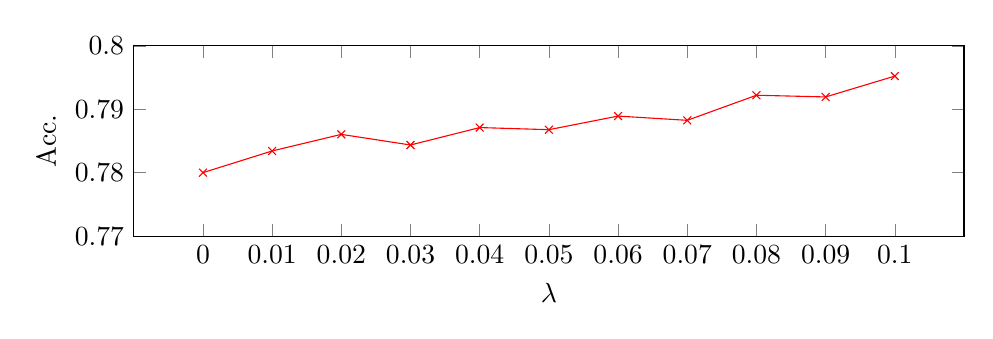
\begin{tikzpicture}
			\begin{axis}[xtick={0,0.01,...,0.1},width=\textwidth,height=4cm,, tick label style={/pgf/number format/fixed},xlabel=$\lambda$,ylabel=Acc.,ymin=0.77,ymax=0.8 ]
				\addplot[color=red,mark=x] coordinates {

					(0, 0.78001876)
					(0.01, 0.78343608)
					(0.02, 0.78604932)
					(0.03, 0.78437416)
					(0.04,  0.78712142)
					(0.05, 0.78678638)
					(0.06, 0.78893058)
					(0.07, 0.78826052)
					(0.08, 0.79221388)
					(0.09, 0.79194586)
					(0.10, 0.79522916)
				};
			\end{axis}
		\end{tikzpicture}
		\caption{The test accuracy of the prediction algorithm under relaxed equalized odds.}
		\label{fig:eqodds}
	\end{figure}
	
	\item Discuss potential limitations of post-processing algorithms.
	
	\textbf{Answer:} Post-processing algorithms don't give useful guarantees about fairness for individuals. E.g., if the post-processing algorithm satisfies Equal Opportunity, then we
know that the true positive rate will be equal across groups, i.e, on expectation a group won't be discriminated against. But that does not give guarantees about the classifier for an individual. Another limitation is that it requires the access to the sensitive attribute which can jeopardise privacy.
\end{enumerate}

\section{Negative feedback loops}
During the task you've calculated several metrics. Fill out the table below. Here, let
\begin{align*}
	X_1 &= \mathbb{P}\left[\frac{\lambda_A}{\lambda_A + \lambda_B}-0.1< \text{ Police's belief without intervention } <\frac{\lambda_A}{\lambda_A + \lambda_B}+0.1\right] \\
	X_2 &= \mathbb{P}\left[\frac{\lambda_A}{\lambda_A + \lambda_B}-0.1< \text{ Police's belief with intervention } <\frac{\lambda_A}{\lambda_A + \lambda_B}+0.1\right] 
\end{align*}

\begin{center}
	\begin{tabular}{r r r r r r  r }
		\toprule
		$\lambda_A$ & $\lambda_B$  &$w_r$ & Historic $A$ & Historic $B$ &  $X_1$ & $X_2$  \\
		\midrule
		0.1 & 0.10 & 0.0 & 10 & 10 & 0.6402 & 1\\
		0.1 & 0.10 & 0.0 & 15 & 5 & 0.069 & 0.9998\\
		0.1 & 0.11 & 0.0 & 10 & 10 & 0.5989 & 0.9999\\
		0.1 & 0.11 & 0.0 & 15 & 5 & 0.1327 & 0.9998\\
		0.1 & 0.10 & 0.9 & 15 & 5 & 1 & 1\\
		\bottomrule
	\end{tabular}
\end{center}


Discuss the influence the initial belief has on the final belief of the police.\\

\textbf{Answer:}
If the initial belief of the police is biased towards a particular neighbourhood A (because historically more crimes were committed in that neighbourhood), the police will go to neighbourhood A more frequently than B - thereby discovering more crimes in A, and in turn strengthening their bias towards neighbourhood A over time. This feedback loop will thus skew the probabilities. \\


Describe your intervention.\\

\textbf{Answer:} On every 2nd day, we make the police ignore the histories of crimes. As a result they are forced to go to the opposite neighbourhood on that day, e.g., if the police were supposed to go to A, now they are forced to go to B - regardless of the history of crime rate. Thus, their belief of crimes observed will update over time more close to the actual rate. This happens because their bias against a certain neighbourhood from an initial belief starts to weaken after observations.



\section{Delayed impact of fair machine learning}
\newcommand{\A}{\mathsf{A}}
\newcommand{\B}{\mathsf{B}}
\newcommand{\TPR}{\text{TPR}}
\newcommand{\maxUtil}{\texttt{maxUtil}}
\newcommand{\DemParity}{\texttt{DP}}
\newcommand{\EqOpp}{\texttt{EO}}
\begin{enumerate}
	\item  Write down the constraints for a policy to satisfy demographic parity and equal opportunity in this setting.
	
	\textbf{Answer:}
        \begin{enumerate}
            \item Demographic parity: 
            $ \sum\limits_{\substack{x \in \chi, \tau_A \leq x}} \pi_A(x) = \sum\limits_{x \in \chi, \tau_B \leq x} \pi_B(x) $

            \item Equal opportunity: $ \frac{\sum\limits_{\substack{x \in \chi, \tau_A \leq x}} \pi_A(x) \rho(x)}{\sum\limits_{\substack{x \in \chi}} \pi_A(x) \rho(x)} = \frac{\sum\limits_{\substack{x \in \chi, \tau_B \leq x}} \pi_B(x) \rho(x)}{\sum\limits_{\substack{x \in \chi}} \pi_B(x) \rho(x)} $
        \end{enumerate}
	
	
	\item Compare the average change of the mean score of the two groups under the
	different conditions.
	
	\textbf{Answer:}
	\begin{center}
		\begin{tabular}{l c c}
			\toprule
			& $\Delta\mu_A$ & $\Delta\mu_B$ \\
			\midrule 
			\maxUtil & 489.15 & 3809.32\\
			\DemParity & 256.79 & 281.40\\
			\EqOpp & 988.39 & 3055.18\\
			\bottomrule
		\end{tabular}
	\end{center}
	
	
	\item Let $\A$ be the underprivileged group, $\tau^*_\A, \beta^*_\A$ be the optimal policy and selection rate for group $\A$ (according to $\Delta\mu_\A$). Assume that $u(x)\geq 0 \Rightarrow \Delta(x) \geq0$. Show that $0 \leq \Delta\mu_\A(\tau^{\text{maxUtil}}_\A) \leq \Delta\mu_\A(\tau^*_\A)$. That means that the policy cannot cause active harm. 
	
	
	\textbf{Answer:} Bank's objective:
    $$ \text{ max } U(r^{-1}(\beta)) = \text{ max } \{g_A\int_{r^{-1}_{\pi_\A}(\beta) \leq x} \pi_A(x)u(x)dx + g_B\int_{r^{-1}_{\pi_\B}(\beta) \leq x} \pi_B(x)u(x)dx\} $$

    Differentiate it wrt $\beta_A$:

    $$ \frac{\partial U(r^{-1}(\beta))}{\partial \beta_A} = -g_A \cdot \pi_A(r^{-1}_{\pi_\A}(\beta)) \cdot u(r^{-1}_{\pi_\A}(\beta)) \cdot \frac{\partial r^{-1}_{\pi_\A}(\beta)}{\partial \beta_A} $$

    $$ =  g_A \cdot u(r^{-1}_{\pi_\A}(\beta)) $$

    We know that $u(x)$ is monotonically increasing. Thus, to maximize utility, the bank will select a $\tau^{maxUtil}_A$ such that $u(\tau^{maxUtil}_A) = 0$. Also, $u(x)\geq 0 \Rightarrow \Delta(x) \geq0$.

    $$ \Delta\mu_\A(\tau^{\text{maxUtil}}_\A) = \int_{\tau_A \leq x} \pi_A(x) \Delta(x) \geq 0$$

    Moreover, by definition, $\Delta\mu_\A(\tau^{\text{maxUtil}}_\A) \leq \Delta\mu_\A(\tau^*_\A)$.
	
	\item Let $\beta \in [0,1]$ with $\beta_\B^\maxUtil> \beta > \beta_\A^\maxUtil$ be fixed, show that there exists a population proportion $g_0$ such that, for all $g_\A \in [0,g_0], \beta_A^\DemParity > \beta $. In particular if $\Delta\mu_\A(r^{-1}_{\pi_\A}(\beta)=0)$ demographic parity causes active harm (i.e. reducing the mean score of group $\A$.).
	
	\textbf{Answer:} Bank's objective:
    $$ \text{ max } U(r^{-1}(\beta)) = \text{ max } \{g_A\int_{r^{-1}_{\pi_\A}(\beta) \leq x} \pi_A(x)u(x)dx + g_B\int_{r^{-1}_{\pi_\B}(\beta) \leq x} \pi_B(x)u(x)dx\} $$

    with Demographic Parity constraint:
    $$ \int_{r^{-1}_{\pi_\A}(\beta) \leq x} \pi_A(x)dx = \int_{r^{-1}_{\pi_\B}(\beta) \leq x} \pi_B(x)dx $$

    Demographic Parity means that both groups have equal selection rate $\Rightarrow$ A and B have the same $\beta$. Differentiating wrt $\beta$ and equating it to 0:

    $$ \frac{\partial U(r^{-1}(\beta))}{\partial \beta} = g_A u(r^{-1}_{\pi_\A}(\beta)) + (1 - g_A) u(r^{-1}_{\pi_\B}(\beta)) = 0 $$

    $$ \Rightarrow g_0 = \frac{u(r^{-1}_{\pi_\B}(\beta))}{u(r^{-1}_{\pi_\B}(\beta)) - u(r^{-1}_{\pi_\A}(\beta))} $$

    Let $g_A = k \cdot g_0, k \in [0, 1]$. Substituting $g_0$ with $g_A$:

    $$ \frac{\partial U(r^{-1}(\beta))}{\partial \beta} = k \cdot g_0 u(r^{-1}_{\pi_\A}(\beta)) + (1 - k \cdot g_0) u(r^{-1}_{\pi_\B}(\beta)) $$

    $$ =  u(r^{-1}_{\pi_\B}(\beta) (1 - k) > 0, \forall k \in [0, 1] $$

    This means that demographic parity will select a $\beta^{DP} > \beta$. If $\Delta \mu_A(r^{-1}_{\pi_\A}(\beta)) = 0$, then by the concave behaviour of $\Delta \mu$ wrt $\beta$, any new $\beta^{DP}$ selected will cause active harm.
	

	\item Use the code provided in  \texttt{Assignment05\_Task04.ipynb} to find a hypothetical $g_0$ such that demographic parity causes active harm to group $\A$.
	
	
	\textbf{Answer:} $g_0 = 0.0115$
\end{enumerate}

\end{document}
